% Created by tikzDevice version 0.6.2-92-0ad2792 on 2013-01-08 03:49:56
% !TEX encoding = UTF-8 Unicode
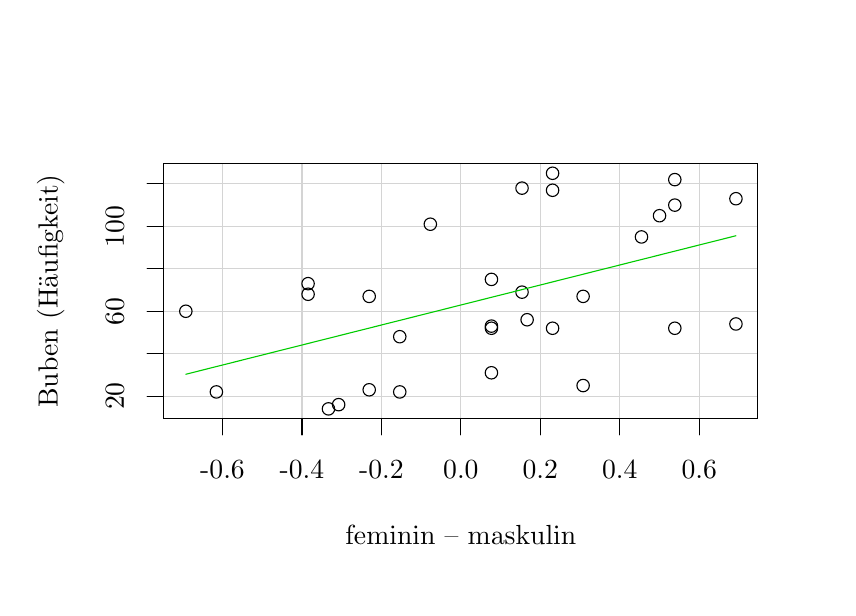
\begin{tikzpicture}[x=1pt,y=1pt]
\definecolor[named]{fillColor}{rgb}{1.00,1.00,1.00}
\path[use as bounding box,fill=fillColor,fill opacity=0.00] (0,0) rectangle (289.08,202.36);
\begin{scope}
\path[clip] (  0.00,  0.00) rectangle (289.08,202.36);
\definecolor[named]{drawColor}{rgb}{0.00,0.00,0.00}

\path[draw=drawColor,line width= 0.4pt,line join=round,line cap=round] ( 70.40, 61.20) -- (242.68, 61.20);

\path[draw=drawColor,line width= 0.4pt,line join=round,line cap=round] ( 70.40, 61.20) -- ( 70.40, 55.20);

\path[draw=drawColor,line width= 0.4pt,line join=round,line cap=round] ( 99.12, 61.20) -- ( 99.12, 55.20);

\path[draw=drawColor,line width= 0.4pt,line join=round,line cap=round] (127.83, 61.20) -- (127.83, 55.20);

\path[draw=drawColor,line width= 0.4pt,line join=round,line cap=round] (156.54, 61.20) -- (156.54, 55.20);

\path[draw=drawColor,line width= 0.4pt,line join=round,line cap=round] (185.25, 61.20) -- (185.25, 55.20);

\path[draw=drawColor,line width= 0.4pt,line join=round,line cap=round] (213.96, 61.20) -- (213.96, 55.20);

\path[draw=drawColor,line width= 0.4pt,line join=round,line cap=round] (242.68, 61.20) -- (242.68, 55.20);

\node[text=drawColor,anchor=base,inner sep=0pt, outer sep=0pt, scale=  1.00] at ( 70.40, 39.60) {-0.6};

\node[text=drawColor,anchor=base,inner sep=0pt, outer sep=0pt, scale=  1.00] at ( 99.12, 39.60) {-0.4};

\node[text=drawColor,anchor=base,inner sep=0pt, outer sep=0pt, scale=  1.00] at (127.83, 39.60) {-0.2};

\node[text=drawColor,anchor=base,inner sep=0pt, outer sep=0pt, scale=  1.00] at (156.54, 39.60) {0.0};

\node[text=drawColor,anchor=base,inner sep=0pt, outer sep=0pt, scale=  1.00] at (185.25, 39.60) {0.2};

\node[text=drawColor,anchor=base,inner sep=0pt, outer sep=0pt, scale=  1.00] at (213.96, 39.60) {0.4};

\node[text=drawColor,anchor=base,inner sep=0pt, outer sep=0pt, scale=  1.00] at (242.68, 39.60) {0.6};

\path[draw=drawColor,line width= 0.4pt,line join=round,line cap=round] ( 49.20, 69.21) -- ( 49.20,145.91);

\path[draw=drawColor,line width= 0.4pt,line join=round,line cap=round] ( 49.20, 69.21) -- ( 43.20, 69.21);

\path[draw=drawColor,line width= 0.4pt,line join=round,line cap=round] ( 49.20, 84.55) -- ( 43.20, 84.55);

\path[draw=drawColor,line width= 0.4pt,line join=round,line cap=round] ( 49.20, 99.89) -- ( 43.20, 99.89);

\path[draw=drawColor,line width= 0.4pt,line join=round,line cap=round] ( 49.20,115.23) -- ( 43.20,115.23);

\path[draw=drawColor,line width= 0.4pt,line join=round,line cap=round] ( 49.20,130.57) -- ( 43.20,130.57);

\path[draw=drawColor,line width= 0.4pt,line join=round,line cap=round] ( 49.20,145.91) -- ( 43.20,145.91);

\node[text=drawColor,rotate= 90.00,anchor=base,inner sep=0pt, outer sep=0pt, scale=  1.00] at ( 34.80, 69.21) {20};

\node[text=drawColor,rotate= 90.00,anchor=base,inner sep=0pt, outer sep=0pt, scale=  1.00] at ( 34.80, 99.89) {60};

\node[text=drawColor,rotate= 90.00,anchor=base,inner sep=0pt, outer sep=0pt, scale=  1.00] at ( 34.80,130.57) {100};

\path[draw=drawColor,line width= 0.4pt,line join=round,line cap=round] ( 49.20, 61.20) --
	(263.88, 61.20) --
	(263.88,153.16) --
	( 49.20,153.16) --
	( 49.20, 61.20);
\end{scope}
\begin{scope}
\path[clip] (  0.00,  0.00) rectangle (289.08,202.36);
\definecolor[named]{drawColor}{rgb}{0.00,0.00,0.00}

\node[text=drawColor,anchor=base,inner sep=0pt, outer sep=0pt, scale=  1.00] at (156.54, 15.60) {feminin -- maskulin};

\node[text=drawColor,rotate= 90.00,anchor=base,inner sep=0pt, outer sep=0pt, scale=  1.00] at ( 10.80,107.18) {Buben (Häufigkeit)};
\end{scope}
\begin{scope}
\path[clip] ( 49.20, 61.20) rectangle (263.88,153.16);
\definecolor[named]{drawColor}{rgb}{0.83,0.83,0.83}

\path[draw=drawColor,line width= 0.4pt,line join=round,line cap=round] ( 70.40, 61.20) -- ( 70.40,153.16);

\path[draw=drawColor,line width= 0.4pt,line join=round,line cap=round] ( 99.12, 61.20) -- ( 99.12,153.16);

\path[draw=drawColor,line width= 0.4pt,line join=round,line cap=round] (127.83, 61.20) -- (127.83,153.16);

\path[draw=drawColor,line width= 0.4pt,line join=round,line cap=round] (156.54, 61.20) -- (156.54,153.16);

\path[draw=drawColor,line width= 0.4pt,line join=round,line cap=round] (185.25, 61.20) -- (185.25,153.16);

\path[draw=drawColor,line width= 0.4pt,line join=round,line cap=round] (213.96, 61.20) -- (213.96,153.16);

\path[draw=drawColor,line width= 0.4pt,line join=round,line cap=round] (242.68, 61.20) -- (242.68,153.16);

\path[draw=drawColor,line width= 0.4pt,line join=round,line cap=round] ( 49.20, 69.21) -- (263.88, 69.21);

\path[draw=drawColor,line width= 0.4pt,line join=round,line cap=round] ( 49.20, 84.55) -- (263.88, 84.55);

\path[draw=drawColor,line width= 0.4pt,line join=round,line cap=round] ( 49.20, 99.89) -- (263.88, 99.89);

\path[draw=drawColor,line width= 0.4pt,line join=round,line cap=round] ( 49.20,115.23) -- (263.88,115.23);

\path[draw=drawColor,line width= 0.4pt,line join=round,line cap=round] ( 49.20,130.57) -- (263.88,130.57);

\path[draw=drawColor,line width= 0.4pt,line join=round,line cap=round] ( 49.20,145.91) -- (263.88,145.91);
\end{scope}
\begin{scope}
\path[clip] (  0.00,  0.00) rectangle (289.08,202.36);
\definecolor[named]{drawColor}{rgb}{0.00,0.00,0.00}

\path[draw=drawColor,line width= 0.4pt,line join=round,line cap=round] ( 49.20, 61.20) --
	(263.88, 61.20) --
	(263.88,153.16) --
	( 49.20,153.16) --
	( 49.20, 61.20);
\end{scope}
\begin{scope}
\path[clip] ( 49.20, 61.20) rectangle (263.88,153.16);
\definecolor[named]{drawColor}{rgb}{0.00,0.00,0.00}

\path[draw=drawColor,line width= 0.4pt,line join=round,line cap=round] (167.58, 93.75) circle (  2.25);

\path[draw=drawColor,line width= 0.4pt,line join=round,line cap=round] (134.45, 70.74) circle (  2.25);

\path[draw=drawColor,line width= 0.4pt,line join=round,line cap=round] (134.45, 90.69) circle (  2.25);

\path[draw=drawColor,line width= 0.4pt,line join=round,line cap=round] (178.63,144.38) circle (  2.25);

\path[draw=drawColor,line width= 0.4pt,line join=round,line cap=round] (178.63,106.79) circle (  2.25);

\path[draw=drawColor,line width= 0.4pt,line join=round,line cap=round] (200.71,105.26) circle (  2.25);

\path[draw=drawColor,line width= 0.4pt,line join=round,line cap=round] (228.32,134.41) circle (  2.25);

\path[draw=drawColor,line width= 0.4pt,line join=round,line cap=round] (108.69, 64.61) circle (  2.25);

\path[draw=drawColor,line width= 0.4pt,line join=round,line cap=round] (167.58, 94.52) circle (  2.25);

\path[draw=drawColor,line width= 0.4pt,line join=round,line cap=round] ( 68.19, 70.74) circle (  2.25);

\path[draw=drawColor,line width= 0.4pt,line join=round,line cap=round] (167.58,111.40) circle (  2.25);

\path[draw=drawColor,line width= 0.4pt,line join=round,line cap=round] (112.37, 66.14) circle (  2.25);

\path[draw=drawColor,line width= 0.4pt,line join=round,line cap=round] (200.71, 73.04) circle (  2.25);

\path[draw=drawColor,line width= 0.4pt,line join=round,line cap=round] (233.84, 93.75) circle (  2.25);

\path[draw=drawColor,line width= 0.4pt,line join=round,line cap=round] (180.47, 96.82) circle (  2.25);

\path[draw=drawColor,line width= 0.4pt,line join=round,line cap=round] (123.41, 71.51) circle (  2.25);

\path[draw=drawColor,line width= 0.4pt,line join=round,line cap=round] (167.58, 77.65) circle (  2.25);

\path[draw=drawColor,line width= 0.4pt,line join=round,line cap=round] (145.50,131.34) circle (  2.25);

\path[draw=drawColor,line width= 0.4pt,line join=round,line cap=round] (189.67, 93.75) circle (  2.25);

\path[draw=drawColor,line width= 0.4pt,line join=round,line cap=round] (101.32,106.03) circle (  2.25);

\path[draw=drawColor,line width= 0.4pt,line join=round,line cap=round] (255.93,140.55) circle (  2.25);

\path[draw=drawColor,line width= 0.4pt,line join=round,line cap=round] (101.32,109.86) circle (  2.25);

\path[draw=drawColor,line width= 0.4pt,line join=round,line cap=round] (233.84,138.24) circle (  2.25);

\path[draw=drawColor,line width= 0.4pt,line join=round,line cap=round] ( 57.15, 99.89) circle (  2.25);

\path[draw=drawColor,line width= 0.4pt,line join=round,line cap=round] (189.67,149.75) circle (  2.25);

\path[draw=drawColor,line width= 0.4pt,line join=round,line cap=round] (233.84,147.45) circle (  2.25);

\path[draw=drawColor,line width= 0.4pt,line join=round,line cap=round] (189.67,143.61) circle (  2.25);

\path[draw=drawColor,line width= 0.4pt,line join=round,line cap=round] (255.93, 95.29) circle (  2.25);

\path[draw=drawColor,line width= 0.4pt,line join=round,line cap=round] (221.80,126.74) circle (  2.25);

\path[draw=drawColor,line width= 0.4pt,line join=round,line cap=round] (123.41,105.26) circle (  2.25);
\definecolor[named]{drawColor}{rgb}{0.00,0.80,0.00}

\path[draw=drawColor,line width= 0.4pt,line join=round,line cap=round] ( 57.15, 77.12) --
	(255.93,127.17);
\end{scope}
\end{tikzpicture}
